\section{Model Optimization}
\label{sec:optimizerStrategies}

When analyzing the range of values obtainable by a model, frequently a key question is ``what set of
parameters result in the best response value?''  To answer this question, RAVEN uses the \xmlNode{Optimizer},
a powerful sampler-like entity that searches the input space to find minimum or maximum values of a response.

In the remainder of this section, we will explore how to use the optimizer using a simple analytic problem,
with a two-dimensional input space and single response of interest.  After getting used to running with the
optimizer, we will add increasing complexity, including changing adaptive step sizes, initial conditions,
parallel trajectories, input space subdivision, input space constraints, and response constraints.

To demonstrate the operation of the Optimizer entities in RAVEN, the model we consider is the Beale function,
which is documented in the analytic tests for RAVEN and replicated here:

\begin{itemize}
  \item Function: $f(x,y) = (1.5-x+xy)^2+(2.25-x+xy^2)^2+(2.625-x+xy^3)^2$
  \item Domain: $-4.5 \leq x,y \leq 4.5$
  \item Global Minimum: $f(3,0.5)=0$
\end{itemize}

The two inputs are the variables $x$ and $y$, and the response is a value we'll assign to $ans$, short for
``answer''.  The model is an external model in RAVEN, and can be found at
\begin{verbatim}
  raven/tests/framework/AnalyticModes/optimizing/beale.py.
\end{verbatim}
The function's values are distributed as in Fig. \ref{fig:beale}, with red indicating high values
and blue indicating low values.
\begin{figure}[h!]
  \centering
  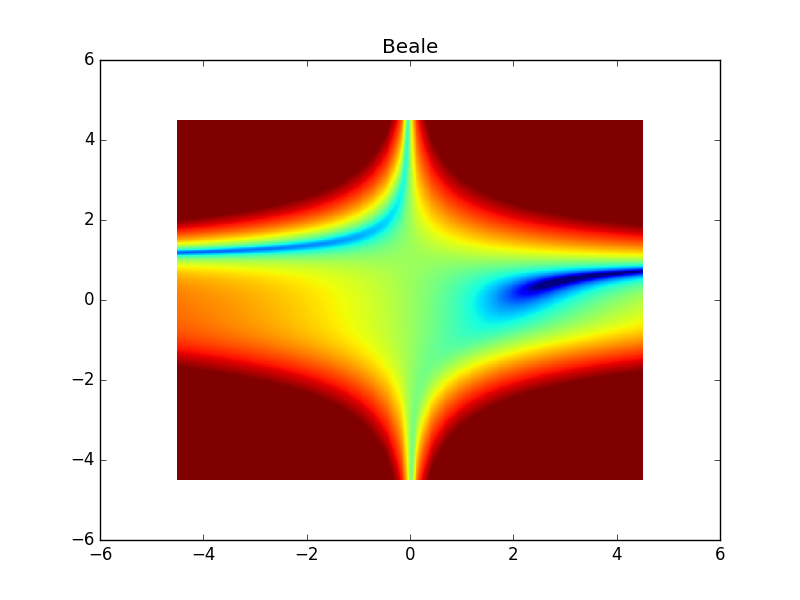
\includegraphics[scale=0.7]{../../tests/framework/user_guide/optimizing/Beale_grid.png}
  \caption{Plot of Beale's function for Optimization}
  \label{fig:beale}
\end{figure}
The objective is to minimize the function.

Note that throughout this example we use the SPSA optimizer by way of demonstration, since it is the first
advanced algorithm for optimization included in RAVEN; many of the options and parameters apply to other
optimizers, and details can be found in the RAVEN user manual.

\subsection{Introduction: The Optimizer Input}
As with other entities, the Optimizer gets its own XML block in the RAVEN input.
Here's an example of an input for a SPSA optimizer named \xmlString{opter}:
\xmlExample{framework/user_guide/optimizing/simple.xml}{Optimizers}
This is the smallest amount of input needed to run an optimization problem, with the exception that we include
the \xmlNode{initialSeed} to maintain consistent results.  Note the required blocks included
to define the optimizer:
\begin{itemize}
  \item \xmlNode{objective}, which is where you indicate the variable for which you want to find the minimum (or,
    if you change the default, maximum).  As listed here, we want to minimize the value of \texttt{ans} given a
    range of possible values for \texttt{x} and \texttt{y}.
  \item \xmlNode{variable}, which is where you can define the input space variables, one for each of these
    nodes.  Declaring a variable here informs the optimizer that you want it to find the optimal value for
    this variable, along with the other variables declared in their own blocks. Note this follows
    the same pattern as any other \xmlNode{Sampler}, including a \xmlNode{distribution} node to
    describe the domain of the variable. For \xmlNode{GradientDescent}, the shape of the
    distribution is not significant unless performing other advanced optimizations (such as
    optimization at risk). Nominally, this distribution simply defines the acceptable range of the
    variable, making the \xmlNode{Uniform} distribution a common choice. The distribution sets the
    upper and lower bounds of the variable, which will give the optimizer some general expectations for
    finding the optimal point; it will never try to sample a value smaller than the lower bound or larger than
    the upper bound.  In the example we define variables \emph{x} and \emph{y} as our input variables, and
    both of them coincidentally range between -4.5 and 4.5.  We set the initial values for both variables to 0
    through the \xmlNode{initial} block, which is required in most cases; the exception is when a
    preconditioner sets them in mulitlevel optimization, but we're not concerned with that feature
    for this example.
  \item \xmlNode{TargetEvaluation}, which declares the DataObject that the optimization search evaluations are
    going to be placed in.  All of the optimal points found as part of the optimization, as well as any other
    points evaluated as part of the algorithm, are placed in this object so the optimizer can retrieve this
    information later.  When this data object is defined, it is critical that the objective variable is
    defined in the output space, and the input variables in the input space, so the optimizer can collect the
    results of its sampling.  The data object type should be ``PointSet'' for this data object.  In this
    example, we use the self-descriptive \emph{optOut} data object.
  \item \xmlNode{samplerInit}, which contains initialization parameters for the optimization
    algorithm. In this case, we set an \xmlNode{initialSeed} to 1234 just to maintain consistent
    results. We also set the maximum number of model evaluations through the \xmlNode{limit} node.
    We don't expect to need all these runs, but in case the optimizer is struggling, we set this
    cutoff to prevent the code running ad infinitum.
  \item \xmlNode{gradient}, which defines the gradient approximation algorithm to use within the
    gradient descent algorithm. In this case,
    we simply indicate that we want to use \xmlNode{SPSA}, and need no additional inputs.
  \item \xmlNode{stepSize}, which defines how we should control the step size during the gradient
    descent algorithm. There are several algorithms to choose from; in this case, we choose
    \xmlNode{GradientHistory}, which uses the scalar product between successive steps to determine
    what step to take in the search algorithm. A bigger growth factor results in traversing the input space more
    quickly, but converging more slowly. A bigger shrink factor results in collapsing to a minimum
    more quickly, converging quickly but possibly falling into local minima. We're using the default
    growth (1.25) and shrink (1.15) factors here.
  \item \xmlNode{acceptance}, which determines the algorithm by which we decide whether to accept a
    potential new optimal point during the gradient descent algorithm. In this case we use
    \xmlNode{Strict}, which indicates any potential new optimal points in the search that are not
    preferrable to the previously-found optimal point are discarded, and the search continues from
    the previously-found optimal point in the search.
  \item \xmlNode{convergence}, which informs the searching algorithm of when to decide it has found
    the optimal point within a sufficient tolerance. There are several stopping criteria; in this
    case, we use the local value of the \xmlNode{gradient}, which we want to be at most 0.1.
\end{itemize}
The other critical blocks in this input are as follows:

\subsubsection{Models}
\xmlExample{framework/user_guide/optimizing/simple.xml}{Models}
Note that we define the external model with the name \xmlString{beale} and provide a path to the analytic
model itself.  This model is set up with the \texttt{run} method that allows RAVEN to run the model.  We also
list all our input/output variables, \emph{x, y}, and \emph{ans}.

\subsubsection{Data Objects}
\xmlExample{framework/user_guide/optimizing/simple.xml}{DataObjects}
We have three data objects:
\begin{itemize}
\item \xmlString{placeholder}, which is necessary to define the input to our external
model in the Steps (the external model doesn't use any input file, so we just use a placeholder
here);
\item \xmlString{optOut}, which will hold all of the samples taken by our optimizer (optimal
candidates, gradient evaluation points, rejected points, etc); and
\item \xmlString{opt\_export}, which will hold the actual solution path taken by our optimizer.  We store the
path travelled by the optimization algorithm as successive samples, with \texttt{iteration} keeping track of the
optimization steps taken.  Note especially how the input of \xmlString{opt\_export} is set to \texttt{trajID},
which is a special keyword for the Optimizer trajectory tracking, as is the output variable \texttt{iteration}.
There are several other special keyword outputs that can be written to the Solution Export data object, that
can be found in the user manual.
\end{itemize}

\subsubsection{Out Streams}
\xmlExample{framework/user_guide/optimizing/simple.xml}{OutStreams}
Here we define the way to print the output of our optimization algorithm.  There's not much to note, except
that we'll be printing the optimization path as a CSV.

\subsubsection{Steps}
\xmlExample{framework/user_guide/optimizing/simple.xml}{Steps}
Here we put it all together into a work flow that RAVEN can follow.  We only need two steps: one to optimize,
and one to print out the results.  To actually perform the optimization, we need a MultiRun step, which we
cleverly name \xmlString{optimize}.  For input we take the placeholder data object \emph{placeholder}, which sets
up the input space of the model we defined, \emph{beal}.  Where a \xmlNode{Sampler} would normally go, we
include the \xmlNode{Optimizer} we defined earlier.  We output to the same data object we indicated in the
Optimizer's \xmlNode{TargetEvaluation} node.  Finally, we note specifically the use of the
\xmlNode{SolutionExport} node.  The data object defined in this node is where the Optimizer will write the
optimization path history, with the final entry being the last step taken by the optimizer.  The IOStep is
unremarkable, used simply to write out the optimization path history to file.

\subsubsection{Conclusion}
After reviewing the components (don't forget the RunInfo block!), you can run this example and see the
results.  In particular, we can view the final results of the optimizer in \texttt{Simple/opt\_export\_0.csv}.  Note
that \texttt{opt\_export} is the name of the \xmlNode{Print} OutStream we defined in the input file.

When we open the file (preferably in a CSV reader such a spreadsheet viewer), we see a CSV with several headers,
the outputs defined in the data object in the input
file: \emph{trajID}, \emph{iteration}, \emph{x}, \emph{y}, and \emph{ans} (not necessarily in that order).  \emph{x},
\emph{y}, and \emph{ans} are the values of the variable at each optimization iteration, while
\emph{iteration} gives the sequential order of the optimization iteration. \emph{trajID} is the
trajectory identifying number; since we are only using one trajectory, this identifier is simply 0.

We can see there's only one line of data in the ouput CSV, showing the final solution discovered by
the optimization algorithm.
If we look at the line, we converged around $f(2.7, 0.42) = 0.0199$ in 40 steps, which is okay but still a little
ways from the analytic optimal point $f(3, 0.5) = 0$.  If we look at the output from the run, we can look at
the last time RAVEN was ``Checking convergence for Trajectory 0''.  Below that statement, there are a series
of convergence criteria and their respeective statuses.  We can see our convergence criteria
requested through the input file (\texttt{gradient}, whose final accepted value is 0.0857) as well
as the \texttt{same point} convergence criteria, which helps determine if the optimal solution is at
a boundary even though other conditions have not converged.

We can see that the reason we converged at the end is the
\texttt{gradient}, which means the relative change in the gradient of \emph{ans} was sufficiently
small between steps to cause convergence.  Clearly, we claimed convergence prematurely because of
the low value required in the optimizer input.  Because these convergence criteria are very
problem-specific, one set parameters will not work best for all problems.

We can improve this result by changing convergence
parameters as well as step size growth and shrink factors, all of which can be found in the user manual, and
many of which we'll discuss in the rest of this section. Feel free to experiment with these values,
and see their affect on the solution discovered.

\subsection{Increasing verbosity}
We saw in the previous section that the output stored in \texttt{Simple/opt\_export.csv} only
includes the final optimal solution, and minimal information about that point. We can increase the
output to see the entire path traversed by adding a few parameters in the input file.

The first parameter to add is in \xmlNode{Optimizers} \xmlNode{GradientDescent}
\xmlNode{samplerInit}. By adding the node \xmlNode{writeSteps} with the value \xmlString{every}, we
can see the full path taken by the optimizer from initial point to final accepted solution.

Further, the optimizer has some special variables that can be use in the \xmlNode{SolutionExport}
\xmlNode{DataObject} to print additional information to the CSV. For example, the special variable
\texttt{accepted} will tell us, for each point in the optimization path, what the result of that
point is. For SPSA, these acceptance notes can be one of the following:
\begin{itemize}
  \item \texttt{first}, or the initial point at which the optimization search begins;
  \item \texttt{accepted}, if the new proposed point is sufficiently improved to be accepted as a
    new optimal point in the search;
  \item \texttt{rejected}, if the new proposed point is \emph{not} sufficiently improved and
    therefore rejected;
  \item \texttt{rerun}, indicating the search algorithm returned to an old optimal point after
    rejecting a proposed optimal point; and
  \item \texttt{final}, which shows that the point listed is the final accepted and converged
    optimal point.
\end{itemize}



\subsection{Initial Conditions and Parallel Trajectories} \label{subsec:opt parallel traj}
Notice we set the optimization search to start at $(0,0)$.
You can change this initial value through
the \xmlNode{initial} block within the \xmlNode{variable} definition nodes.

Furthermore, RAVEN offers the possibility to run multiple optimization paths in parallel.  Because many
(perhaps most) optimization techniques get stuck in local minima, using multiple paths (or \emph{trajectories} as
they are called in RAVEN) increases the likelihood that one of the trajectories will find the global minimum
point.  You can request multiple trajectories by providing a variety of initial conditions in the
\xmlNode{initial} block, as shown in this Optimizer example:
\xmlExample{framework/user_guide/optimizing/multiple_trajectories.xml}{Optimizers}
Note that the ordered pairs are split across the \xmlNode{initial} nodes, so that the first trajectory will
start as a point made up of all the first entries, the second trajectory starts at all the second entries, and
et cetera.  In this case, we've requested starting points at (-2,-2), (-2,2), (2,-2), and (2,2).  This (and
defining a new working directory in the \xmlNode{RunInfo} block) is the only input change between the original
file and this one.

When run, we can see the results in the working directory \texttt{MultipleTraj}.  There, we see the same files
as for the base case, plus \texttt{opt\_export} files 0-3.  These are produced because we've
clustered the outputs by \texttt{trajID} in the \xmlNode{OutStreams} definition. Each of these corresponds to the
path that one of the initial points started at, as you can see at the top of each of these CSV files.  We can
see that trajectory 2 (who started at (2,-2)) ended close to the analytic optimal point, while trajectory 1
was far from it.

In the screen output from the RAVEN run, you can see the final summary shows the status of each
trajectory. Under \emph{Trajectory Results} we see trajectories 1-3 all converged with different
optimal values, while trajectory 0 is marked as \emph{following 1}. This means at some point
Trajectory 0 started following the same path as Trajectory 1 already moved along, so Trajectory 0
was terminated as a result to save computational resources.

Finally, we see the optimal point selected was Trajectory 2 with a function value of roughly 3.7e-3
at (3.15, 0.54).

\subsection{Adjusting Adaptive Steps} \label{subsec:opt stepsize}
As we've seen, some of the optimization paths are struggling to converge to meaningful optimal solutions.
One way to improve this is to tinker with the convergence tolerances as shown in the user manual.  Another is
to change the step size modifications used as part of the search process, which we discuss in this section.
First, we briefly discuss how the SPSA chooses its step size, so we can make informed choices about what
parameters to use.

Because SPSA is a gradient-based method, it operates by starting at a particular point, estimating the
gradient at that point, then taking a step in the opposite direction of the gradient in order to follow a
downhill path.  It adaptively chooses how long of a step to take based on its history.  If the gradient is in
the same direction twice in a row, the algorithm assumes there's further to travel, so increases its step size
multiplicatively by the \emph{growthFactor}, which we had defaulted to 1.25.  If, on the other hand,
the gradient switches directions, then the step size is divided by the \emph{shrinkFactor}, which we
had defaulted to 1.15.  This means that by default, if the gradient keeps going in the same direction, you
always increase your step size by 25\%, while if you're bouncing back and forth in a valley, the
step size is reduced by 15\% at each iteration.

By way of note, in higher dimensions, the actual growth or shrink multiplier is scaled by a dot product
between the two previous gradients, with a max of the grain growth factor when the dot product is 1 (exactly
aligned) and a minimum of grain shrink factor when the dot product is -1 (exactly opposite).  This means if
the gradient is at right angles with the past gradient, then the step size remains unchanged (dot product is
0).

There are some additional considerations for the step size change, as well.  If the algorithm takes a step,
then discovers the new point has a worse response value than the point it's at, it will reject the new point,
re-evaluate the gradient, and flag the step size to be divided by the gain shrink factor.  Because of this, if
the gain shrink factor is too large, false convergence can be obtained when the algorithm struggles to find a
new downhill point to move to.  As a result, in practice it is often beneficial to have a gain shrink factor
that is smaller than the gain growth factor.

For this new example, we use gain growth factor of 1.25 (meaning when the gradient continues in the same
direction our step grows by 25\% of its old value) and a gain shrink factor of 1.1 (meaning when the
gradient flips directions our step size shrinks to 90\% of its old value).  We add this to the base case
(\texttt{simple.xml}) to get:
\xmlExample{framework/user_guide/optimizing/step_size.xml}{Optimizers}
Note the definition of the gain growth and shrink factors in the \xmlNode{convergence} block.  Reviewing the
output file \texttt{StepSize}, we can see more steps were taken than the case using default step sizes, but
the final solution was $f(2.75,0.430)=0.013$ in 40 iterations, which is closer to the analytical solution of $f(3,0.5)=0$
than the original case using the same number of iterations.

It is often challenging to find the best gain growth and shrink factors, and these can have a very significant
impact on the speed and accuracy of the convergence process.  Too large a shrink factor results in poor
resolution of valleys, while too small a shrink factor results in many unnecessary evaluations of the model.

% TODO rewrite with new sampler-based denoising options
% \subsection{Denoising Stochastic Problems}
% While many of the models we see in optimization are deterministic (meaning running the same inputs into the
% model yields the same results every time), there are quite a few stochastic models that we might desire to
% optimize.  For example, a model that included Brownian motion or is solved using unseeded random numbers might
% be considered stochastic.

% The difficulty with optimizing noisy problems rests in the unreliability of a single sample.  If we send a
% single set of inputs into a stochastic model, we can't trust the results to be consistent.  One way to measure
% the consistency of the results is through a signal-to-noise ratio (SNR).  There are many ways to define this
% value; for our purposes, we will use the ratio of the mean of the signal to the standard deviation of the
% signal, $\mu/\sigma$.

% To obtain an approximation of your SNR, you can use RAVEN to perform a Monte Carlo run on your model and then
% use the BasicStatistics postprocessor to collect the mean (expectedValue) and standard deviation (sigma) of
% your response.  It's important to make this sampling all at a single value in the input space, so replace your
% variables with constants in the Sampler input.  Once you have the mean and sigma, you have an idea of how
% noisy your model is.  A SNR of 1 means the signal is just as big as the noise, making it very difficult to
% optimize.  A SNR of less than 1 means the noise dominates the signal, and will make optimization almost
% impossible without introducing denoising.  A SNR of more than 1 indicates the signal is stronger than the
% noise, and perhaps denoising is not necessary.  If your standard deviation is 0, then you don't have any
% discernable noise!

% To denoise a model in RAVEN SPSA optimization currently, we turn our attention to the \xmlNode{Optimizer}
% subnode \xmlNode{parameter}, specifically the \xmlNode{numGradAvgIterations} node.  This parameter instructs
% RAVEN to perform multiple gradient evaluations, including multiple evaluations of each optimal point, and use
% the average to make decisions in optimization pathing.  By default, RAVEN takes one optimal point and one
% neighboring point to evaluate a gradient.  Increasing the \xmlNode{numGradAvgIterations} will increase the
% number of times the optimal point is sampled, and how many neighbor points are sampled.  This serves to
% denoise the model.

% However, this also raises the question, how many resamples do I need to denoise my model?  In a Wilks-like
% approach, we want to reduce the size of the confidence interval for our mean to be less than the noise.  The
% number of resamples required depends on the size of the confidence interval $z$ and the confidence-to-noise ratio
% $\xi$ we want to ultimately have for the optimization algorithm.  We also assume the distribution of the
% response is roughly Gaussian Normal, which may not be the case.  The approximate equation for assuring the
% confidence interval is smaller than the noise is
% \begin{equation}
%   \frac{z\sigma}{\sqrt{n}} \leq \xi\sigma,
% \end{equation}
% \begin{equation}
%   n \geq \left(\frac{z}{\xi}\right)^2.
% \end{equation}
% Thus, the number of resamples depends on the confidence level as well as the desired ratio of the confidence interval
% to the noise.

% A few values for varying ratios are given in Table \ref{tab:confidence levels} for the 99\% confidence level ($z=2.576$).
% \begin{table}[htb]
%   \centering
%   \begin{tabular}{c c}
%     Confidence-to-noise $\xi$ & Resamples necessary \\ \hline
%     1.0 & 7 \\
%     0.9 & 9 \\
%     0.7 & 14 \\
%     0.5 & 27 \\
%     0.1 & 664 \\
%     0.05 & 2655
%   \end{tabular}
%   \caption{Estimate of the number of samples necessary to denoise models to varying confidence levels}
%   \label{tab:confidence levels}
% \end{table}
% That is, if you want the noise and confidence interval to have the same magnitude, only 7 resamples are
% required.  If, on the other hand, you want the confidence interval to be half the level of the noise, 27
% resamples are required.

% Note these are only guidelines; individual models may behave differently and require more or less resamples to
% provide a clear optimization path.

\subsection{Functional Constraints} \label{subsec:opt explicit constraint}
Sometimes an optimization problem has a constrained input space, possibly where there is a tradeoff between
two inputs.  In this event, RAVEN allows the user to define a \emph{constraint} function, which will cause
RAVEN to treat this constraint as it would a boundary condition.

For example, we will introduce a void in the input where we reject inputs.  This void is defined by rejecting
all samples within $(x-1)^2 + y^2 < 1$.  We'll also include the modified step growth and shrink parameters
discussed in section \ref{subsec:opt stepsize}.

To include a constraint function, we first have to define it in the RAVEN input as a \xmlNode{Function}
entity:
\xmlExample{framework/user_guide/optimizing/constrain.xml}{Functions}
Note that the file \texttt{./Constrain/constraint.py} is located relative to the working directory.  Currently,
external functions are always Python files.  In that file,
note that the only method is \texttt{constrain}, which is RAVEN's keyword to find the constraint function.
RAVEN will pass in a \texttt{self} object, which will have the function variables defined in the
\xmlNode{Functions} input available as members.  The method \texttt{constrain} then returns a boolean which is \texttt{True} if
the evaluation does not violate the constraint, or \texttt{False} if the constraint is violated.

To attach the constraint to the optimizer, simply add it as an assembled \xmlNode{Function}:
\xmlExample{framework/user_guide/optimizing/constrain.xml}{Optimizers}

After running, looking through the path followed by trajectory 0 shows that instead of following the path from
section \ref{subsec:opt stepsize}, the path moves to lower \emph{y} values before swinging back up toward the
optimal point.

%\subsection{Implicit Constraints (Penalties)}
% TODO come up with a working example
